% Options for packages loaded elsewhere
\PassOptionsToPackage{unicode}{hyperref}
\PassOptionsToPackage{hyphens}{url}
%
\documentclass[
  10pt,
  ignorenonframetext,
]{beamer}
\usepackage{pgfpages}
\setbeamertemplate{caption}[numbered]
\setbeamertemplate{caption label separator}{: }
\setbeamercolor{caption name}{fg=normal text.fg}
\beamertemplatenavigationsymbolsempty
% Prevent slide breaks in the middle of a paragraph
\widowpenalties 1 10000
\raggedbottom
\setbeamertemplate{part page}{
  \centering
  \begin{beamercolorbox}[sep=16pt,center]{part title}
    \usebeamerfont{part title}\insertpart\par
  \end{beamercolorbox}
}
\setbeamertemplate{section page}{
  \centering
  \begin{beamercolorbox}[sep=12pt,center]{part title}
    \usebeamerfont{section title}\insertsection\par
  \end{beamercolorbox}
}
\setbeamertemplate{subsection page}{
  \centering
  \begin{beamercolorbox}[sep=8pt,center]{part title}
    \usebeamerfont{subsection title}\insertsubsection\par
  \end{beamercolorbox}
}
\AtBeginPart{
  \frame{\partpage}
}
\AtBeginSection{
  \ifbibliography
  \else
    \frame{\sectionpage}
  \fi
}
\AtBeginSubsection{
  \frame{\subsectionpage}
}
\usepackage{lmodern}
\usepackage{amssymb,amsmath}
\usepackage{ifxetex,ifluatex}
\ifnum 0\ifxetex 1\fi\ifluatex 1\fi=0 % if pdftex
  \usepackage[T1]{fontenc}
  \usepackage[utf8]{inputenc}
  \usepackage{textcomp} % provide euro and other symbols
\else % if luatex or xetex
  \usepackage{unicode-math}
  \defaultfontfeatures{Scale=MatchLowercase}
  \defaultfontfeatures[\rmfamily]{Ligatures=TeX,Scale=1}
\fi
% Use upquote if available, for straight quotes in verbatim environments
\IfFileExists{upquote.sty}{\usepackage{upquote}}{}
\IfFileExists{microtype.sty}{% use microtype if available
  \usepackage[]{microtype}
  \UseMicrotypeSet[protrusion]{basicmath} % disable protrusion for tt fonts
}{}
\makeatletter
\@ifundefined{KOMAClassName}{% if non-KOMA class
  \IfFileExists{parskip.sty}{%
    \usepackage{parskip}
  }{% else
    \setlength{\parindent}{0pt}
    \setlength{\parskip}{6pt plus 2pt minus 1pt}}
}{% if KOMA class
  \KOMAoptions{parskip=half}}
\makeatother
\usepackage{xcolor}
\IfFileExists{xurl.sty}{\usepackage{xurl}}{} % add URL line breaks if available
\IfFileExists{bookmark.sty}{\usepackage{bookmark}}{\usepackage{hyperref}}
\hypersetup{
  pdftitle={GKN 2020-2021: Contactmoment 6},
  pdfauthor={Tine van Daal \& Sofie Vermeiren},
  hidelinks,
  pdfcreator={LaTeX via pandoc}}
\urlstyle{same} % disable monospaced font for URLs
\newif\ifbibliography
\usepackage{color}
\usepackage{fancyvrb}
\newcommand{\VerbBar}{|}
\newcommand{\VERB}{\Verb[commandchars=\\\{\}]}
\DefineVerbatimEnvironment{Highlighting}{Verbatim}{commandchars=\\\{\}}
% Add ',fontsize=\small' for more characters per line
\usepackage{framed}
\definecolor{shadecolor}{RGB}{248,248,248}
\newenvironment{Shaded}{\begin{snugshade}}{\end{snugshade}}
\newcommand{\AlertTok}[1]{\textcolor[rgb]{0.94,0.16,0.16}{#1}}
\newcommand{\AnnotationTok}[1]{\textcolor[rgb]{0.56,0.35,0.01}{\textbf{\textit{#1}}}}
\newcommand{\AttributeTok}[1]{\textcolor[rgb]{0.77,0.63,0.00}{#1}}
\newcommand{\BaseNTok}[1]{\textcolor[rgb]{0.00,0.00,0.81}{#1}}
\newcommand{\BuiltInTok}[1]{#1}
\newcommand{\CharTok}[1]{\textcolor[rgb]{0.31,0.60,0.02}{#1}}
\newcommand{\CommentTok}[1]{\textcolor[rgb]{0.56,0.35,0.01}{\textit{#1}}}
\newcommand{\CommentVarTok}[1]{\textcolor[rgb]{0.56,0.35,0.01}{\textbf{\textit{#1}}}}
\newcommand{\ConstantTok}[1]{\textcolor[rgb]{0.00,0.00,0.00}{#1}}
\newcommand{\ControlFlowTok}[1]{\textcolor[rgb]{0.13,0.29,0.53}{\textbf{#1}}}
\newcommand{\DataTypeTok}[1]{\textcolor[rgb]{0.13,0.29,0.53}{#1}}
\newcommand{\DecValTok}[1]{\textcolor[rgb]{0.00,0.00,0.81}{#1}}
\newcommand{\DocumentationTok}[1]{\textcolor[rgb]{0.56,0.35,0.01}{\textbf{\textit{#1}}}}
\newcommand{\ErrorTok}[1]{\textcolor[rgb]{0.64,0.00,0.00}{\textbf{#1}}}
\newcommand{\ExtensionTok}[1]{#1}
\newcommand{\FloatTok}[1]{\textcolor[rgb]{0.00,0.00,0.81}{#1}}
\newcommand{\FunctionTok}[1]{\textcolor[rgb]{0.00,0.00,0.00}{#1}}
\newcommand{\ImportTok}[1]{#1}
\newcommand{\InformationTok}[1]{\textcolor[rgb]{0.56,0.35,0.01}{\textbf{\textit{#1}}}}
\newcommand{\KeywordTok}[1]{\textcolor[rgb]{0.13,0.29,0.53}{\textbf{#1}}}
\newcommand{\NormalTok}[1]{#1}
\newcommand{\OperatorTok}[1]{\textcolor[rgb]{0.81,0.36,0.00}{\textbf{#1}}}
\newcommand{\OtherTok}[1]{\textcolor[rgb]{0.56,0.35,0.01}{#1}}
\newcommand{\PreprocessorTok}[1]{\textcolor[rgb]{0.56,0.35,0.01}{\textit{#1}}}
\newcommand{\RegionMarkerTok}[1]{#1}
\newcommand{\SpecialCharTok}[1]{\textcolor[rgb]{0.00,0.00,0.00}{#1}}
\newcommand{\SpecialStringTok}[1]{\textcolor[rgb]{0.31,0.60,0.02}{#1}}
\newcommand{\StringTok}[1]{\textcolor[rgb]{0.31,0.60,0.02}{#1}}
\newcommand{\VariableTok}[1]{\textcolor[rgb]{0.00,0.00,0.00}{#1}}
\newcommand{\VerbatimStringTok}[1]{\textcolor[rgb]{0.31,0.60,0.02}{#1}}
\newcommand{\WarningTok}[1]{\textcolor[rgb]{0.56,0.35,0.01}{\textbf{\textit{#1}}}}
\setlength{\emergencystretch}{3em} % prevent overfull lines
\providecommand{\tightlist}{%
  \setlength{\itemsep}{0pt}\setlength{\parskip}{0pt}}
\setcounter{secnumdepth}{-\maxdimen} % remove section numbering
\usepackage{graphicx}
\usepackage{rotating}

%\setbeamertemplate{caption}[numbered]

\usepackage{hyperref}
\usepackage{caption}
\usepackage[normalem]{ulem}
%\mode<presentation>
\usepackage{wasysym}
\usepackage{amsmath}

\usetheme{Luebeck}
\useoutertheme{miniframes} % Alternatively: miniframes, infolines, split
\useinnertheme{circles}

\setbeamertemplate{navigation symbols}{}
\institute{Opleidings- en onderwijswetenschappen}
\titlegraphic{\includegraphics[width=0.3\paperwidth]{\string edubronlogo.png}}
\setbeamertemplate{title page}[empty]

\setbeamerfont{subtitle}{size=\small}

\setbeamercovered{transparent}

\definecolor{edubronblauw}{RGB}{4,68,102}
\definecolor{edubrongroen}{RGB}{170,170,23}
\definecolor{uarood}{RGB}{147,0,49}

\setbeamercolor{frametitle}{fg=edubronblauw,bg=white}
\setbeamercolor{title}{fg=edubronblauw,bg=white}
\setbeamercolor{subtitle}{fg=edubrongroen,bg=edubronblauw}
\setbeamercolor{local structure}{fg=edubronblauw}
\setbeamercolor{section in toc}{fg=edubronblauw,bg=white}
% \setbeamercolor{subsection in toc}{fg=edubrongroen,bg=white}

\setbeamercolor{item projected}{fg=edubronblauw,bg=white}
\setbeamertemplate{itemize item}{\color{edubronblauw}$\bullet$}
\setbeamertemplate{itemize subitem}{\color{uarood}\scriptsize{$\bullet$}}

\setbeamercolor{palette primary}{bg=edubronblauw,fg=white}
\setbeamercolor{palette secondary}{bg=edubronblauw,fg=white}
\setbeamercolor{palette tertiary}{bg=edubronblauw,fg=white}
\setbeamercolor{palette quaternary}{bg=edubronblauw,fg=white}
\setbeamercolor{subsection in head/foot}{bg=edubrongroen,fg=white}

\let\Tiny=\tiny

\def\begincols{\begin{columns}}
\def\begincol{\begin{column}}
\def\endcol{\end{column}}
\def\endcols{\end{columns}}

\AtBeginPart{}
\AtBeginSection{}
\AtBeginSubsection{}
\AtBeginSubsubsection{}
\setlength{\emergencystretch}{0em}
\setlength{\parskip}{0pt}

\title{GKN 2020-2021: Contactmoment 6}
\subtitle{Logistische regressie-analyse (2)}
\author{Tine van Daal \& Sofie Vermeiren}
\date{}

\begin{document}
\frame{\titlepage}

\begin{frame}
  \tableofcontents[hideallsubsections]
\end{frame}
\hypertarget{recap}{%
\section{Recap}\label{recap}}

\begin{frame}{}
\protect\hypertarget{section}{}

\textcolor{uarood}{Recap}

\end{frame}

\begin{frame}[fragile]{Laatste model vorig contactmoment}
\protect\hypertarget{laatste-model-vorig-contactmoment}{}

\tiny

\begin{verbatim}

Call:
glm(formula = Onderpresteren ~ Gender + Ouders_GraagLezenZ, family = binomial(), 
    data = Vlaanderen_1_2_3)

Deviance Residuals: 
    Min       1Q   Median       3Q      Max  
-1.1701  -0.6869  -0.5991  -0.4531   2.2943  

Coefficients:
                   Estimate Std. Error z value Pr(>|z|)    
(Intercept)        -1.37641    0.05319  -25.88  < 2e-16 ***
GenderGirls        -0.25424    0.07611   -3.34 0.000836 ***
Ouders_GraagLezenZ -0.39405    0.03856  -10.22  < 2e-16 ***
---
Signif. codes:  0 '***' 0.001 '**' 0.01 '*' 0.05 '.' 0.1 ' ' 1

(Dispersion parameter for binomial family taken to be 1)

    Null deviance: 4496.7  on 4634  degrees of freedom
Residual deviance: 4377.4  on 4632  degrees of freedom
  (563 observations deleted due to missingness)
AIC: 4383.4

Number of Fisher Scoring iterations: 4
\end{verbatim}

\normalsize

\end{frame}

\begin{frame}{Effect van `Ouders\_GraagLezenZ'}
\protect\hypertarget{effect-van-ouders_graaglezenz}{}

\begincols
  \begincol{.48\textwidth}
\begin{center}
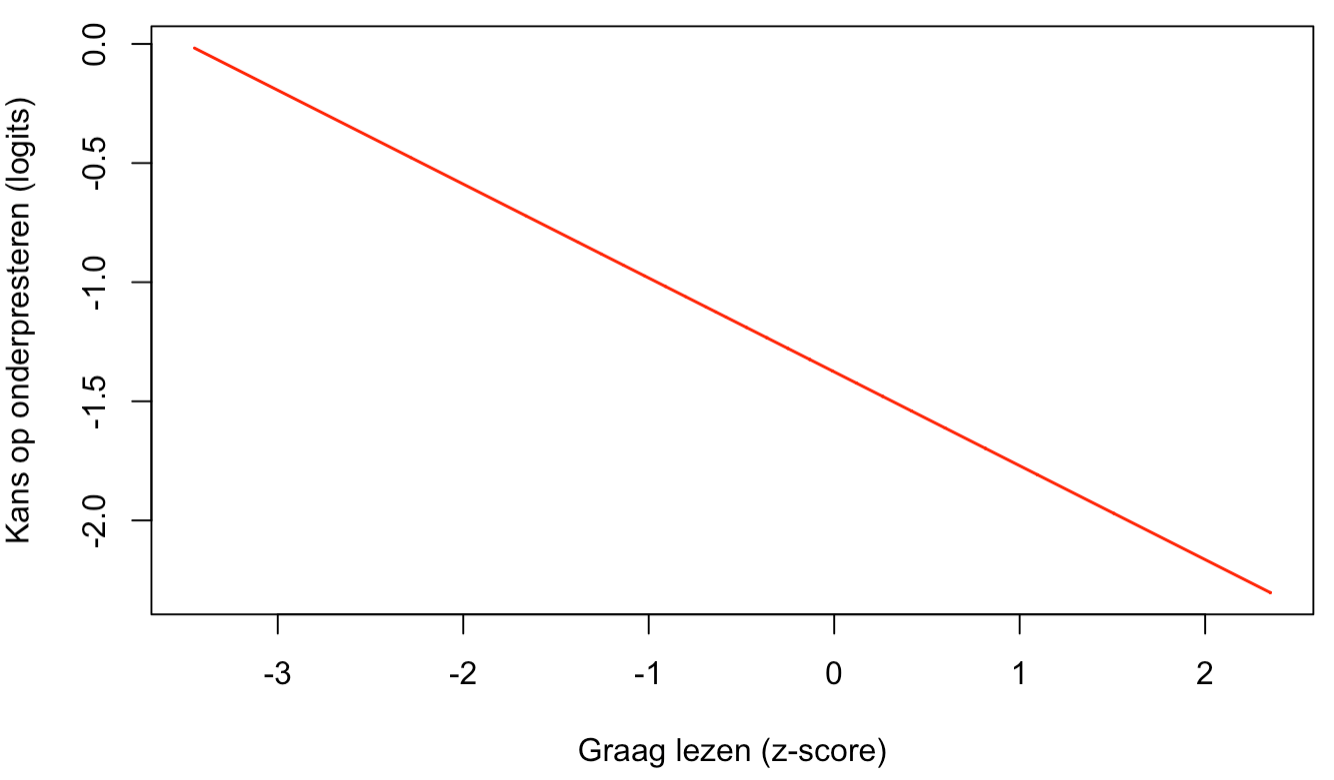
\includegraphics[width=0.95\textwidth]{PlotLOG.png}
\end{center}
\endcol
  \begincol{.48\textwidth}
  \begin{center}
\includegraphics[width=0.95\textwidth]{PlotPROB.png}
\end{center}
\endcol
\endcols

\end{frame}

\begin{frame}[fragile]{Effect van `Gender'}
\protect\hypertarget{effect-van-gender}{}

\tiny

\begin{Shaded}
\begin{Highlighting}[]
\KeywordTok{library}\NormalTok{(sjPlot)}
\KeywordTok{plot_model}\NormalTok{(M1_PIRLS, }\DataTypeTok{transform =} \OtherTok{NULL}\NormalTok{, }\DataTypeTok{type =} \StringTok{"eff"}\NormalTok{, }\DataTypeTok{terms =} \KeywordTok{c}\NormalTok{(}\StringTok{"Gender"}\NormalTok{))}
\end{Highlighting}
\end{Shaded}

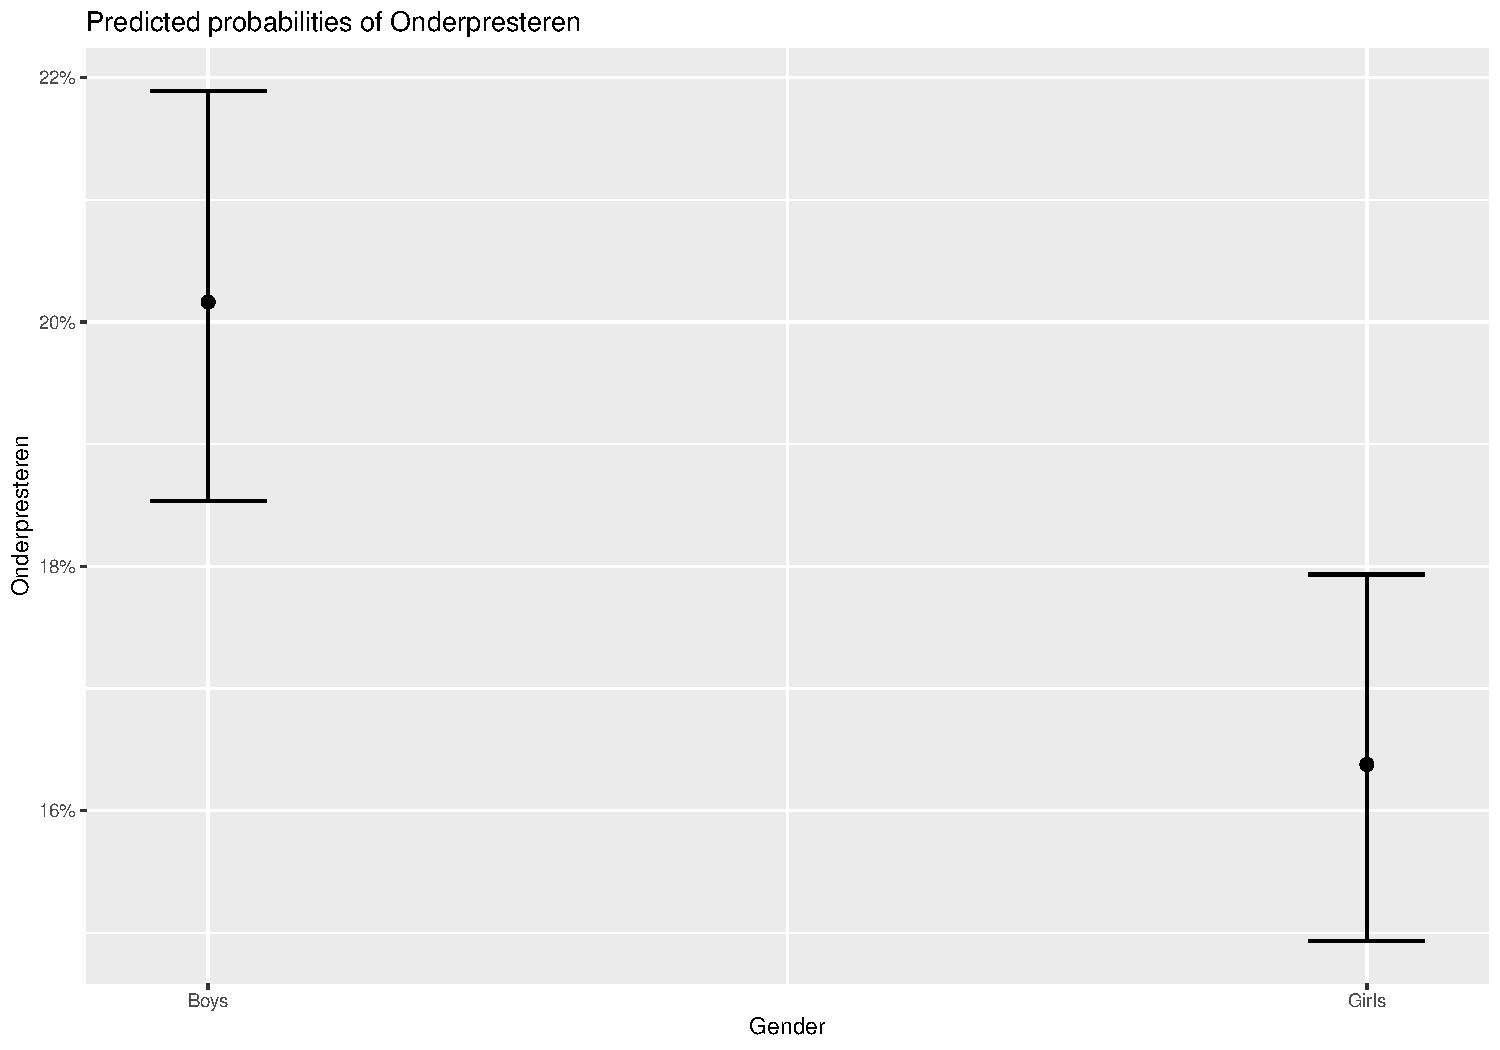
\includegraphics[height=0.7\textheight]{C6_files/figure-beamer/unnamed-chunk-4-1}

\normalsize

\end{frame}

\begin{frame}[fragile]{Beide effecten samen?}
\protect\hypertarget{beide-effecten-samen}{}

\tiny

\begin{Shaded}
\begin{Highlighting}[]
\KeywordTok{plot_model}\NormalTok{(M1_PIRLS, }\DataTypeTok{transform =} \OtherTok{NULL}\NormalTok{, }\DataTypeTok{type =} \StringTok{"eff"}\NormalTok{, }\DataTypeTok{terms =} \KeywordTok{c}\NormalTok{(}\StringTok{"Ouders_GraagLezenZ"}\NormalTok{, }\StringTok{"Gender"}\NormalTok{))}
\end{Highlighting}
\end{Shaded}

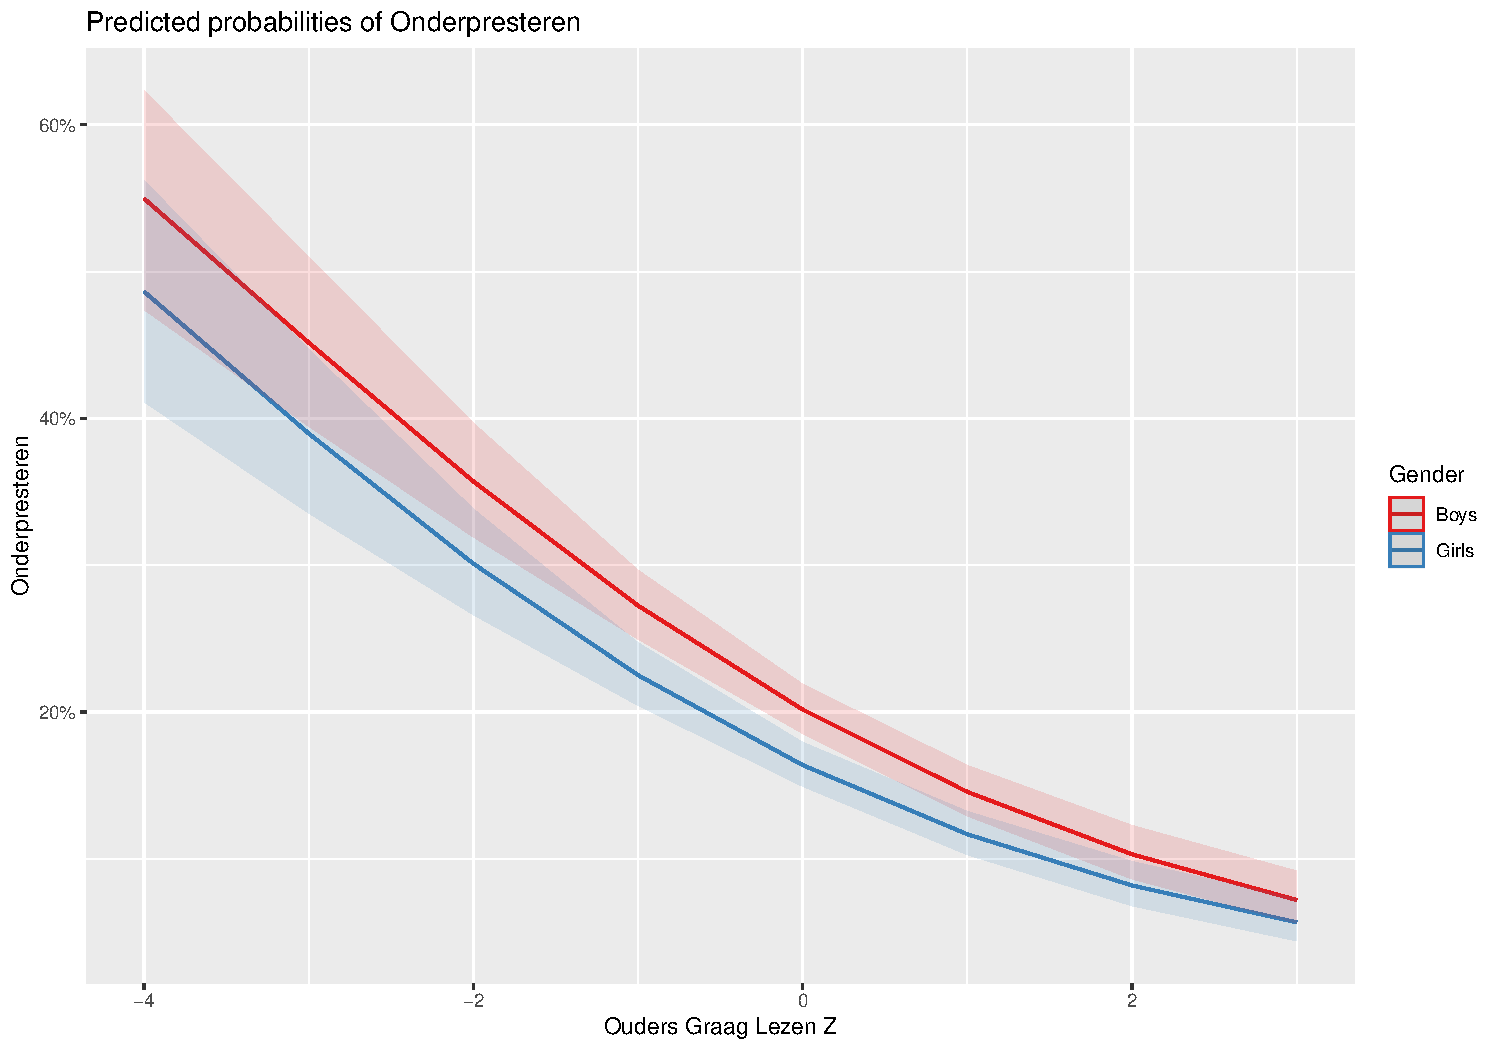
\includegraphics[height=0.7\textheight]{C6_files/figure-beamer/unnamed-chunk-5-1}

\normalsize

\end{frame}

\hypertarget{odds}{%
\section{Odds}\label{odds}}

\begin{frame}{}
\protect\hypertarget{section-1}{}

\textcolor{uarood}{Let's talk in Odds}

\end{frame}

\begin{frame}[fragile]{Parameters als Odds interpreteren (1)}
\protect\hypertarget{parameters-als-odds-interpreteren-1}{}

\[Logit(Onderpr. = 1 ) = \] \[-1.376 +
  (-0.254*GenderGirl) + (-0.394*OudersLezenZ)  \]

\tiny

\begin{Shaded}
\begin{Highlighting}[]
\KeywordTok{exp}\NormalTok{(}\OperatorTok{-}\FloatTok{1.376}\NormalTok{)}
\end{Highlighting}
\end{Shaded}

\begin{verbatim}
[1] 0.2525869
\end{verbatim}

\normalsize

\emph{Voor jongens wiens ouders gemiddeld graag lezen is de kans om te
behoren tot de onderpresteerders 0.25 keer groter (of 1/0.25 = 4 keer
kleiner) dan de kans om niet tot de onderpresteerders te behoren}

\end{frame}

\begin{frame}[fragile]{Parameters als Odds interpreteren (2)}
\protect\hypertarget{parameters-als-odds-interpreteren-2}{}

\[ Logit(Onderpr. = 1 ) =\]
\[-1.376 + (-0.254*GenderGirl) + (-0.394*OudersLezenZ) \]

\tiny

\begin{Shaded}
\begin{Highlighting}[]
\KeywordTok{exp}\NormalTok{(}\OperatorTok{-}\FloatTok{0.254}\NormalTok{)}
\end{Highlighting}
\end{Shaded}

\begin{verbatim}
[1] 0.7756918
\end{verbatim}

\begin{Shaded}
\begin{Highlighting}[]
\DecValTok{1}\OperatorTok{/}\KeywordTok{exp}\NormalTok{(}\OperatorTok{-}\FloatTok{0.254}\NormalTok{)}
\end{Highlighting}
\end{Shaded}

\begin{verbatim}
[1] 1.289172
\end{verbatim}

\normalsize

\emph{Voor meisjes wiens ouders gemiddeld graag lezen is de
\textcolor{uarood}{kansverhouding} om te behoren tot de
onderpresteerders eerder dan tot de `niet onderpresteerders' 0.776 keer
groter (of 1/0.776 = 1.289 keer kleiner) dan voor jongens}

\bigskip

0.776 is een \textbf{\textcolor{uarood}{Odds Ratio}}

\end{frame}

\begin{frame}[fragile]{Parameters als Odds interpreteren (3)}
\protect\hypertarget{parameters-als-odds-interpreteren-3}{}

\begin{center}
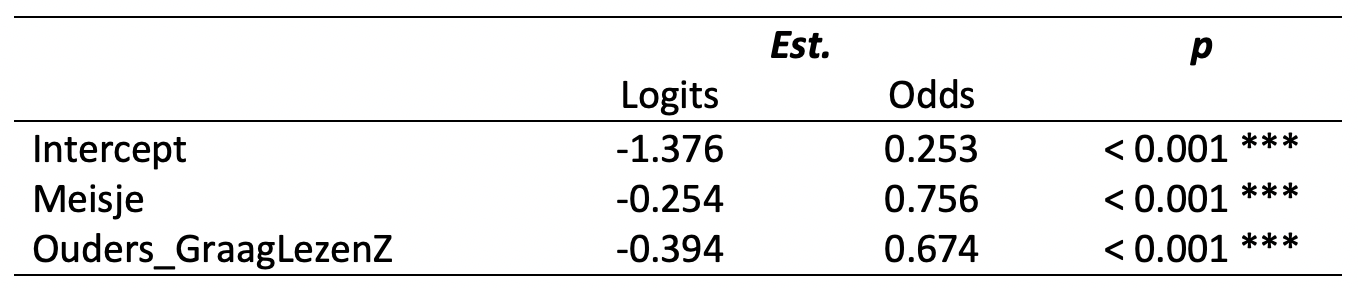
\includegraphics[width=0.75\textwidth]{LogOdds.png}
\end{center}

\bigskip

Voorspelde Odds voor meisjes:

\tiny

\begin{Shaded}
\begin{Highlighting}[]
\CommentTok{## Voorspelde Odds meisjes:}
\KeywordTok{exp}\NormalTok{(}\OperatorTok{-}\FloatTok{1.376}\NormalTok{) }\OperatorTok{*}\StringTok{ }\KeywordTok{exp}\NormalTok{(}\OperatorTok{-}\FloatTok{0.254}\NormalTok{)}
\end{Highlighting}
\end{Shaded}

\begin{verbatim}
[1] 0.1959296
\end{verbatim}

\normalsize \bigskip     Odds zijn \textbf{multiplicatief}

\end{frame}

\hypertarget{het-ene-model-is-het-andere-niet}{%
\section{Het ene model is het andere
niet}\label{het-ene-model-is-het-andere-niet}}

\begin{frame}{}
\protect\hypertarget{section-2}{}

\textcolor{uarood}{Hoe goed zijn modellen?}

\end{frame}

\begin{frame}{Geen \(R^2\)}
\protect\hypertarget{geen-r2}{}

Bij gewone regressie-analyse hebben we een geschat residu:

\[ Score_{i}= \beta_0 + \beta_1 * x_1 + \beta_2 * x_2 + ... + \epsilon_{ij}\]
\bigskip     Gewone regressieanalyse: \emph{Ordinary Least Squares}
(OLS) schattingen\\
Schattingen die de afstand van de regressielijn met de residuen
minimaliseert!

\end{frame}

\begin{frame}{Maximum Likelihood}
\protect\hypertarget{maximum-likelihood}{}

Bij logistische regressieanalyse hebben we geen geschat residu!

\[ Logit(X=1)= \beta_0 + \beta_1 * x_1 + \beta_2 * x_2 + ... \]
\bigskip     Logistische regressieanalyse:
\textcolor{uarood}{Maximum Likelihood} (ML) schattingen

\end{frame}

\begin{frame}{Maximum Likelihood}
\protect\hypertarget{maximum-likelihood-1}{}

\bigskip

Likelihood = functie van parameterwaarden (gegeven de data)!

\bigskip

Doel: die combinatie van parameterwaarden waarvoor de Likelihood zo hoog
mogelijk is (=Maximaal)

\bigskip

Hoe?

\begin{itemize}
\tightlist
\item
  Likelihood wordt eerst log-getransformeerd
\item
  Via `afgeleiden' van Log-likelihood functie parameterwaarden waarvoor
  de log-likelihood maximaal is
\end{itemize}

\bigskip

\(\rightarrow\) Voor een model krijgen we ook een
\textcolor{uarood}{Log-likelihood (LL)} waarde (= indicatie van FIT!)

\end{frame}

\begin{frame}{Modellen vergelijken}
\protect\hypertarget{modellen-vergelijken}{}

\bigskip

2 concurrerende modellen, welk model zou je weerhouden?

\bigskip

\(\rightarrow\) Model met hoogste waarde voor LL!

\end{frame}

\begin{frame}[fragile]{Nulmodel als start}
\protect\hypertarget{nulmodel-als-start}{}

Nulmodel = model zonder voorspellers

\tiny

\begin{Shaded}
\begin{Highlighting}[]
\NormalTok{M0_PIRLS <-}\StringTok{ }\KeywordTok{glm}\NormalTok{(Onderpresteren }\OperatorTok{~}\StringTok{ }\DecValTok{1}\NormalTok{, }
                \DataTypeTok{data =}\NormalTok{ Vlaanderen_}\DecValTok{1}\NormalTok{_}\DecValTok{2}\NormalTok{_}\DecValTok{3}\NormalTok{, }\DataTypeTok{family =} \KeywordTok{binomial}\NormalTok{())}
\KeywordTok{summary}\NormalTok{(M0_PIRLS)}
\end{Highlighting}
\end{Shaded}

\begin{verbatim}

Call:
glm(formula = Onderpresteren ~ 1, family = binomial(), data = Vlaanderen_1_2_3)

Deviance Residuals: 
    Min       1Q   Median       3Q      Max  
-0.6725  -0.6725  -0.6725  -0.6725   1.7875  

Coefficients:
            Estimate Std. Error z value Pr(>|z|)    
(Intercept) -1.37145    0.03452  -39.73   <2e-16 ***
---
Signif. codes:  0 '***' 0.001 '**' 0.01 '*' 0.05 '.' 0.1 ' ' 1

(Dispersion parameter for binomial family taken to be 1)

    Null deviance: 5236.4  on 5197  degrees of freedom
Residual deviance: 5236.4  on 5197  degrees of freedom
AIC: 5238.4

Number of Fisher Scoring iterations: 4
\end{verbatim}

\normalsize

\end{frame}

\begin{frame}[fragile]{Vergelijking met Model1}
\protect\hypertarget{vergelijking-met-model1}{}

\tiny

\begin{Shaded}
\begin{Highlighting}[]
\KeywordTok{logLik}\NormalTok{(M0_PIRLS)}
\end{Highlighting}
\end{Shaded}

\begin{verbatim}
'log Lik.' -2618.19 (df=1)
\end{verbatim}

\begin{Shaded}
\begin{Highlighting}[]
\KeywordTok{logLik}\NormalTok{(M1_PIRLS)}
\end{Highlighting}
\end{Shaded}

\begin{verbatim}
'log Lik.' -2188.681 (df=3)
\end{verbatim}

\normalsize \bigskip     In onderzoek wordt -2 keer LL gehanteerd (=
\textbf{-2LL} of \textbf{Deviance})

\tiny

\begin{Shaded}
\begin{Highlighting}[]
\KeywordTok{deviance}\NormalTok{(M0_PIRLS)}
\end{Highlighting}
\end{Shaded}

\begin{verbatim}
[1] 5236.379
\end{verbatim}

\begin{Shaded}
\begin{Highlighting}[]
\KeywordTok{deviance}\NormalTok{(M1_PIRLS)}
\end{Highlighting}
\end{Shaded}

\begin{verbatim}
[1] 4377.362
\end{verbatim}

\normalsize

\end{frame}

\begin{frame}[fragile]{Via anova()}
\protect\hypertarget{via-anova}{}

\tiny

\begin{Shaded}
\begin{Highlighting}[]
\KeywordTok{anova}\NormalTok{(M0_PIRLS, M1_PIRLS)}
\end{Highlighting}
\end{Shaded}

\normalsize

\(\rightarrow\)
\texttt{Error\ in\ anova.glmlist(c(list(object),\ dotargs),\ dispersion\ =\ dispersion,\ :\ models\ were\ not\ all\ fitted\ to\ the\ same\ size\ of\ dataset}

\end{frame}

\begin{frame}[fragile]{Vergelijking modellen (invloed van `missing
values')}
\protect\hypertarget{vergelijking-modellen-invloed-van-missing-values}{}

Modellen kunnen enkel vergeleken worden als ze geschat zijn op dezelfde
dataset (en dus ook op evenveel observatie-eenheden)!

\begin{Shaded}
\begin{Highlighting}[]
\KeywordTok{nrow}\NormalTok{(M0_PIRLS}\OperatorTok{$}\NormalTok{model)}
\end{Highlighting}
\end{Shaded}

\begin{verbatim}
[1] 5198
\end{verbatim}

\begin{Shaded}
\begin{Highlighting}[]
\KeywordTok{nrow}\NormalTok{(M1_PIRLS}\OperatorTok{$}\NormalTok{model)}
\end{Highlighting}
\end{Shaded}

\begin{verbatim}
[1] 4635
\end{verbatim}

\(\rightarrow\) Nulmodel herschatten op enkel de 4635 observaties om
model te kunnen vergelijken

\end{frame}

\begin{frame}[fragile]{Vergelijking modellen}
\protect\hypertarget{vergelijking-modellen}{}

Missing values verwijderen: \tiny

\begin{Shaded}
\begin{Highlighting}[]
\NormalTok{Dat_analyse <-}\StringTok{ }\KeywordTok{na.omit}\NormalTok{( Vlaanderen_}\DecValTok{1}\NormalTok{_}\DecValTok{2}\NormalTok{_}\DecValTok{3}\NormalTok{[ , }\KeywordTok{c}\NormalTok{(}\StringTok{"Onderpresteren"}\NormalTok{, }\StringTok{"Gender"}\NormalTok{, }\StringTok{"Ouders_GraagLezenZ"}\NormalTok{)] )}
\end{Highlighting}
\end{Shaded}

\normalsize \medskip     Modellen herschatten: \tiny

\begin{Shaded}
\begin{Highlighting}[]
\NormalTok{M0_PIRLS <-}\StringTok{ }\KeywordTok{glm}\NormalTok{(Onderpresteren }\OperatorTok{~}\StringTok{ }\DecValTok{1}\NormalTok{, }
                \DataTypeTok{data =}\NormalTok{ Dat_analyse, }\DataTypeTok{family =} \KeywordTok{binomial}\NormalTok{())}

\NormalTok{M1_PIRLS <-}\StringTok{ }\KeywordTok{glm}\NormalTok{(Onderpresteren }\OperatorTok{~}\StringTok{ }\NormalTok{Gender }\OperatorTok{+}\StringTok{ }\NormalTok{Ouders_GraagLezenZ, }
                \DataTypeTok{data =}\NormalTok{ Dat_analyse, }\DataTypeTok{family =} \KeywordTok{binomial}\NormalTok{())}
\end{Highlighting}
\end{Shaded}

\normalsize \medskip Modellen vergelijken: \tiny

\begin{Shaded}
\begin{Highlighting}[]
\KeywordTok{anova}\NormalTok{(M0_PIRLS , M1_PIRLS, }\DataTypeTok{test=}\StringTok{"Chi"}\NormalTok{)}
\end{Highlighting}
\end{Shaded}

\begin{verbatim}
Analysis of Deviance Table

Model 1: Onderpresteren ~ 1
Model 2: Onderpresteren ~ Gender + Ouders_GraagLezenZ
  Resid. Df Resid. Dev Df Deviance  Pr(>Chi)    
1      4634     4496.7                          
2      4632     4377.4  2   119.32 < 2.2e-16 ***
---
Signif. codes:  0 '***' 0.001 '**' 0.01 '*' 0.05 '.' 0.1 ' ' 1
\end{verbatim}

\normalsize

\end{frame}

\begin{frame}[fragile]{Vergelijking modellen}
\protect\hypertarget{vergelijking-modellen-1}{}

Stappenplan:

\begin{itemize}
\tightlist
\item
  Nadenken over welke modellen je gaat schatten (gegeven je OV)
\item
  Data-object maken zonder missings voor alle variabelen
  \texttt{na.omit()}
\item
  Alternatieve modellen schatten op aangemaakt data-object
\item
  Modellen vergelijken
\item
  Beste model weerhouden en \textbf{herschatten op je originele dataset}
\item
  Interpretatie (Nadenken over tabellen en figuren)
\end{itemize}

\end{frame}

\end{document}
